\section{eo\-Fitness\-Stat$<$ EOT, Fit\-T $>$ Class Template Reference}
\label{classeo_fitness_stat}\index{eoFitnessStat@{eoFitnessStat}}
The fitnesses of a whole population, as a vector.  


{\tt \#include $<$eo\-MOFitness\-Stat.h$>$}

Inheritance diagram for eo\-Fitness\-Stat$<$ EOT, Fit\-T $>$::\begin{figure}[H]
\begin{center}
\leavevmode
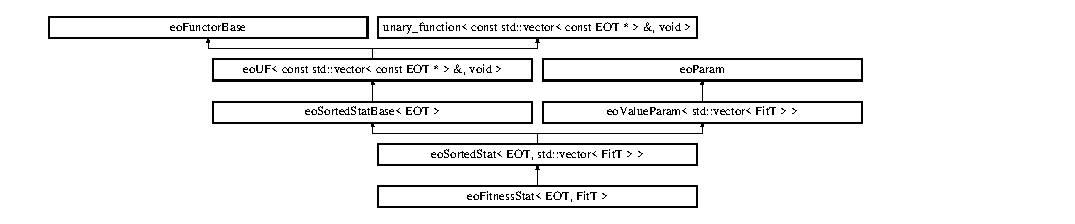
\includegraphics[height=2.55708cm]{classeo_fitness_stat}
\end{center}
\end{figure}
\subsection*{Public Member Functions}
\begin{CompactItemize}
\item 
{\bf eo\-Fitness\-Stat} (std::string \_\-description=\char`\"{}All\-Fitnesses\char`\"{})\label{classeo_fitness_stat_a0}

\item 
virtual void {\bf operator()} (const std::vector$<$ const {\bf EOT} $\ast$ $>$ \&\_\-pop\-Pters)\label{classeo_fitness_stat_a1}

\begin{CompactList}\small\item\em The pure virtual function that needs to be implemented by the subclass. \item\end{CompactList}\end{CompactItemize}


\subsection{Detailed Description}
\subsubsection*{template$<$class EOT, class Fit\-T = typename EOT::Fitness$>$ class eo\-Fitness\-Stat$<$ EOT, Fit\-T $>$}

The fitnesses of a whole population, as a vector. 



Definition at line 36 of file eo\-MOFitness\-Stat.h.

The documentation for this class was generated from the following file:\begin{CompactItemize}
\item 
eo\-MOFitness\-Stat.h\end{CompactItemize}
